\titre{17}
\theme{trigo}
\auteur{Nathan Scheinmann}
\niveau{1M}
\source{sesamath-1M-trigo}
\type{serie}
\piments{2}
\pts{}
\annee{2425}

\contenu{
\tcblower
Pour déterminer la hauteur du Mont Ticule, Sophie a mesuré les angles $\alpha, \beta$ et la distance $d$. Calculer $h$ en sachant que $\alpha=30^\circ, \beta=45^\circ$ et $d=200~\text{m}$. 
\begin{center}
	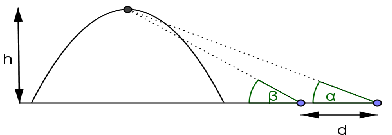
\includegraphics[scale=1]{../medias/1M/trigo/1M-exo-17}
\end{center}
}
\correction{

}

